\documentclass[]{article}
\usepackage{amsmath}
\usepackage{tikz}
\usepackage{listofitems}
\usepackage{etoolbox}

\tikzset{>=latex}
\colorlet{myred}{red!80!black}
\colorlet{myblue}{blue!80!black}
\colorlet{mygreen}{green!60!black}
\colorlet{myorange}{orange!80!black}
\colorlet{myyellow}{yellow!80!black}

\colorlet{mydarkred}{myred!40!black}
\colorlet{mydarkblue}{myblue!40!black}
\colorlet{mydarkgreen}{mygreen!40!black}
\colorlet{mydarkorange}{myorange!40!black}
\colorlet{mydarkyellow}{myyellow!40!black}

\tikzset{
  node/.style={very thick,circle,draw=myblue,minimum size=22,inner sep=0.5,outer sep=0.6},
  input/.style={node,mydarkgreen,draw=mygreen,fill=mygreen!25},
  conv/.style={node,mydarkorange,draw=myorange,fill=myorange!25},
  flat/.style={node,mydarkyellow,draw=myyellow,fill=myyellow!25},
  dense/.style={node,mydarkblue,draw=myblue,fill=myblue!20},
  output/.style={node,mydarkred,draw=myred,fill=myred!20},
  connect/.style={-,thick,mydarkblue,shorten >=1}
}

\def\nstyle{%
  int(\lay==1 ? 1 : % Input
  (\lay<5 ? 2 :      % Conv layers
  (\lay==5 ? 3 :     % Flatten
  (\lay<8 ? 4 : 5))))} % Dense + Output

\begin{document}

\begin{titlepage}
  \centering

  \vspace*{4cm}

  \Huge
  \textbf{Tactibrême}

  \vspace{1cm}

  \huge
  \textbf{Agents et Réseaux de Neurones}

  \vfill

  \Large
  \textbf{Auteurs:} Gros Charlène, Pottier Loïc, Mudoy Jacques, Horter Louise, Los Thomas, Gambier Clément

  \vspace{1cm}

  \textbf{Date de rendu:} \today
  
\end{titlepage}

\tableofcontents

\newpage

\section{Introduction}
Ce document fournit une présentation détaillée des architectures de réseaux de neurones utilisées pour jouer au jeu de plateau `Les tacticiens de Brême`. Il couvre la représentation des données d'entrée, le codage des sorties, le fonctionnement de l'apprentissage par renforcement profond (\textit{Deep Q-Learning}) ainsi que les différentes couches du réseau.
Nous étudierons d'abord le focntionnement du DQL avant de détailler les différents modèles utilisés.

\section{Le DQL}
Le Deep Q-Learning (DQN) est un méthode d'apprentissage par reforcement (Reinforcement Learning) visant à entraîner un agent à interagir avec un environnement pour maximiser une récompense cumulative. L'agent apprend à prendre des décisions en fonction de l'état actuel de l'environnement et des récompenses associées à chaque action. Le DQL est basé sur l'apprentissage profond et utilise un réseau de neurones pour approximer la fonction \(Q(s, a)\), qui estime la récompense attendue pour une action donnée dans un état donné.

\subsection{Utilisation de datasets}
Dans la plupart des applications de l'apprentissage profond, l'entraînement repose sur des ensembles de données statistiques (\textit{offline learning}). Par exemple, les réseaux de neurones convolutionnels (CNN) sont généralement entraînés sur des datasets d'images (\textit{e.g., ImageNet}), tandis que les modèles NLP exploitent des corpus de texte préexistants. De manière similaire, certaines approches de RL exploitent des expériences passées sous forme de datasets pré-enregistrés pour optimiser la politique d'un agent, comme dans l'\textit{Offline Reinforcement Learning}.

\subsection{Apprentissage par récompense}
Dans notre cas particulier, n'ayant pas accès a un dataset, nous adoptons une approche d'apprentissage plus directe. L'agent apprend à jouer en interagissant directement avec l'environnement, en explorant les différentes actions possibles et en ajustant ses stratégies en fonction des récompenses reçues. L'agent est entraîné à maximiser la récompense cumulative en utilisant une combinaison d'exploration aléatoire et d'exploitation des connaissances acquises.

\section{Nécessité de deux modèles: jeu et draft de placement}
Au début d'une partie, les deux joueurs doivent placer leurs pions sur le plateau. Ce placement initial est crucial pour la suite de la partie, car il détermine les options stratégiques disponibles. Chaque joueur doit placer un pion à tour de role jusqu'à ce que les 8 pions soient placés. Pour cette phase de draft, nous utiliserons un modèle spécifique prenant en entrée une représentation partielle du plateau de jeu et produisant une distribution sur les cases disponibles. Ce modèle est entièrement distinct du modèle principal qui sera utilisé pour les mouvements pendant la partie.

\subsection{Pourquoi un modèle séparé ?}
L'apprentissage d'un modèle unique pour l'ensemble du jeu présente plusieurs inconvénients :
\begin{itemize}
    \item \textbf{Différence d'objectifs} : Les objectifs de la phase de draft et de la phase de jeu sont différents. Le modèle de draft doit apprendre à placer les pions de manière stratégique par rapport aux placements adverses, tandis que le modèle de jeu doit apprendre à prendre des décisions tactiques pour gagner la partie.
    \item \textbf{Représentation différente} : La phase de draft nécessite une représentation différente du plateau, car les pions ne sont pas encore placés. Un modèle distinct permet de gérer cette différence de manière plus efficace. Il est inutile d'utiliser les mêmes dimensions d'entrées/sortie pour les deux modèles.
\end{itemize}

\subsection{Approche d'apprentissage}
\begin{itemize}
    \item \textbf{Draft} : L'agent place les pions et est récompensé en fonction de la qualité du placement. La récompense est déterminée en fonction du déroulement de la partie.
    \item \textbf{Jeu} : L'agent prend des décisions pour gagner la partie, en apprenant progressivment à l'aide des récompenses données par l'environnement à chacun de ses mouvements.
\end{itemize}

\section{Modèle 1} % TODO: Si on leur donne des noms c'est sympa
Ce premier modèle prend en entrée une représentation du plateau de jeu et produit une distribution sur les mouvements possibles.
Le modèle n'ayant pas connaissance des mouvements interdits, on utilise un masque pour les éviter.

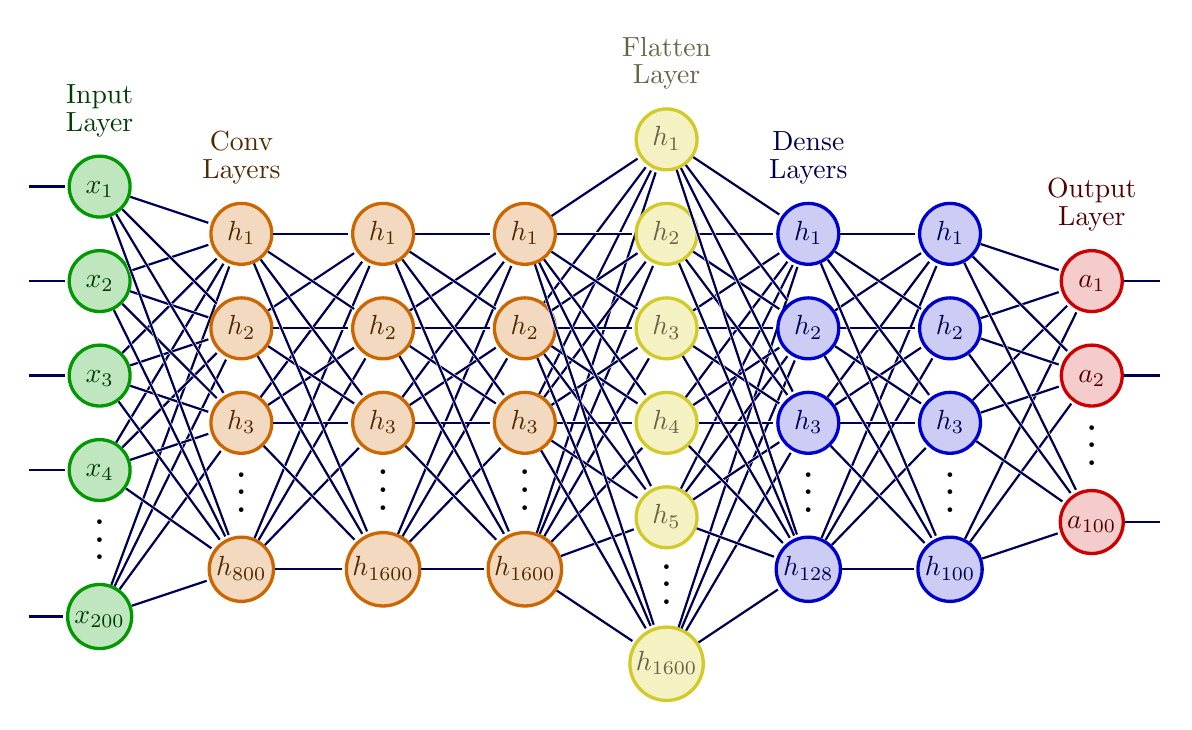
\begin{tikzpicture}[x=1.8cm,y=1.2cm]
    % Input: 5 nodes
    % Conv Layers (2-4): 32, 64, 64 nodes
    % Flatten Layer (5): 1600 nodes
    % Dense Layers (6-7): 128, 100 nodes
    % Output Layer (8): 100 nodes
    \readlist\Nnod{5,4,4,4,6,4,4,3} 
    
    \readlist\Nnode{200, 800, 1600, 1600,1600,128,100,100}  
    \readlist\Cstr{x,h,h,h,a,z,z,y} 
    
    \def\yshift{0.55}
    
    \foreachitem \N \in \Nnod{
        \def\lay{\Ncnt}
        \pgfmathsetmacro\prev{int(\Ncnt-1)}
        \foreach \i [evaluate={
            \c = int(\i==\N);
            \y = \N/2 - \i - \c * \yshift;
            \x = \lay;
            \n = \nstyle;
            \index = (\i<\N ? int(\i) : "\Nnode[\lay]");
        }] in {1,...,\N}{
            \pgfmathsetmacro\nstyle{int(\n==1 ? "input" : (\n==2 ? "conv" : (\n==3 ? "flat" : (\n==4 ? "dense" : "output"))))}
            \node[\nstyle] (N\lay-\i) at (\x,\y) {$\strut\Cstr[\n]_{\index}$};
            \ifnumcomp{\lay}{>}{1}{
                \foreach \j in {1,...,\Nnod[\prev]}{
                    \draw[white,line width=1.2,shorten >=1] (N\prev-\j) -- (N\lay-\i);
                    \draw[connect] (N\prev-\j) -- (N\lay-\i);
                }
                \ifnum \lay=\Nnodlen
                    \draw[connect] (N\lay-\i) --++ (0.5,0);
                \fi
            }{
                \draw[connect] (0.5,\y) -- (N\lay-\i);
            }
        }
        \path (N\lay-\N) --++ (0,1+\yshift) node[midway,scale=1.6] {$\vdots$};
    }
    \node[above=3,align=center,mydarkgreen] at (N1-1.90) {Input\\[-0.2em]Layer};
    \node[above=3,align=center,mydarkorange] at (N2-1.90) {Conv\\[-0.2em]Layers};
    \node[above=3,align=center,mydarkyellow] at (N5-1.90) {Flatten\\[-0.2em]Layer};
    \node[above=3,align=center,mydarkblue] at (N6-1.90) {Dense\\[-0.2em]Layers};
    \node[above=3,align=center,mydarkred] at (N8-1.90) {Output\\[-0.2em]Layer};
\end{tikzpicture}

\subsection{Représentation des Entrées}
Le plateau est représenté comme une grille \(5 \times 5\), où chaque case est encodée par un vecteur à 8 canaux décrivant la présence des différents pions.

\begin{itemize}
    \item Les 4 premiers canaux : Présence des pions bleues (\textit{âne\_bleu}, \textit{chien\_bleu}, \textit{chat\_bleu}, \textit{coq\_bleu}).
    \item Les 4 canaux suivants : Présence des pions rouges (\textit{âne\_rouge}, \textit{chien\_rouge}, \textit{chat\_rouge}, \textit{coq\_rouge}).
\end{itemize}

\paragraph{Exemple}

\begin{verbatim}
[0, 0, 1, 0, 1, 0, 0, 0] # chat bleu, âne rouge
[0, 0, 0, 0, 0, 0, 0, 0] # case vide
\end{verbatim}

\subsubsection{Dimensions des Entrées}
\begin{itemize}
    \item Pour un plateau unique : \((8, 5, 5)\) (canaux, lignes, colonnes).
    \item Pour un lot de plateaux (\textit{batch}) : \((\text{taille\_batch}, 8, 5, 5)\).
\end{itemize}

\subsection{Représentation des Sorties}
La sortie du réseau encode tous les déplacements possibles sous forme de liste aplatie de paires \((\text{pion}, \text{destination})\).

\subsubsection{Taille de la Sortie}
La sortie compte \(4 \times 25 = 100\) mouvements possibles :
\begin{itemize}
    \item 4 pions possibles (par joueur).
    \item 25 cases possibles (une grille \(5 \times 5\)).
\end{itemize}

\subsubsection{Encodage des Placements}
Chaque index \(i\) dans la sortie correspond à :
\[
\text{index\_pion} = \frac{i}{25}, \quad
\text{ligne\_destination} = \frac{i \bmod 25}{5}, \quad
\text{colonne\_destination} = i \bmod 5.
\]

\subsubsection{Masquage}
Un masque binaire est appliqué aux 100 scores de sortie pour invalider les mouvements impossibles. Les mouvements invalides reçoivent un score de \(-\infty\) avant l'étape \textit{softmax} :
\begin{verbatim}
Masque = [0, 1, 0, ..., 1]  # 1 pour les mouvements valides, 0 sinon
\end{verbatim}

\subsection{Architecture du Réseau de Neurones}
L'architecture prend la représentation du plateau en entrée et produit une distribution sur les 100 mouvements possibles. Le réseau utilise des couches convolutionnelles pour extraire les caractéristiques spatiales, suivies de couches entièrement connectées pour produire les scores finaux.

\subsubsection{Entrée}
\(\text{Dimensions d'Entrée}: (\text{taille\_batch}, 8, 5, 5)\)

\subsubsection{Couches Convolutionnelles}
\begin{itemize}
    \item \(\text{Conv2D}(8 \rightarrow 32)\) \(\rightarrow\) ReLU
    \item \(\text{Conv2D}(32 \rightarrow 64)\) \(\rightarrow\) ReLU
    \item \(\text{Conv2D}(64 \rightarrow 64)\) \(\rightarrow\) ReLU
\end{itemize}

\subsubsection{Couches Entièrement Connectées}
\begin{itemize}
    \item \(\text{Flatten}\)
    \item \(\text{Linear}(5 \times 5 \times 64 \rightarrow 128) \rightarrow \text{ReLU}\)
    \item \(\text{Linear}(128 \rightarrow 100)\)
\end{itemize}

\subsubsection{Sortie}
\[
(\text{taille\_batch}, 100)
\]
Ce vecteur est ensuite combiné avec le \textit{masque} pour garantir que seuls les mouvements valides sont pris en compte.

\subsection{Mécanisme de sélection des actions}
Après avoir obtenu les scores pour chaque action possible, l'agent doit sélectionner un mouvement à exécuter. Plutôt que de choisir systématiquement l'action avec le score le plus élevé, nous utilisons une approche probabiliste qui favorise l'exploration tout en privilégiant les actions à fort potentiel.

\subsubsection{Politique stochastique}
Nous convertissons les scores du réseau en une distribution de probabilités à l'aide de la fonction softmax:

\[
P(a_i) = \frac{e^{q_i}}{\sum_j e^{q_j}}
\]

où \(q_i\) est le score attribué à l'action \(i\) par le réseau.

\subsubsection{Échantillonnage multinomial}
Plutôt que de sélectionner l'action avec la probabilité la plus élevée (exploitation pure), nous échantillonnons une action selon la distribution calculée:

\begin{verbatim}
action_index = torch.multinomial(probabilités, 1).item()
\end{verbatim}

Cette approche offre plusieurs avantages:
\begin{itemize}
    \item \textbf{Exploration guidée}: Les actions avec des scores élevés ont plus de chances d'être sélectionnées, mais les actions moins prometteuses peuvent également être explorées.
    \item \textbf{Diversité des stratégies}: L'agent ne joue pas toujours de manière déterministe, ce qui le rend moins prévisible et potentiellement plus robuste.
    \item \textbf{Prévention du sur-ajustement}: La variabilité dans les actions aide à éviter que l'agent se bloque dans des stratégies sous-optimales.
\end{itemize}

\subsubsection{Masquage des actions invalides}
Avant l'application de softmax, les actions invalides sont masquées en assignant une valeur très négative à leurs scores (\(-10^9\)):

\begin{verbatim}
q_values[mask == 0] = -1e9
\end{verbatim}

Cela garantit que leur probabilité après softmax sera pratiquement nulle, les excluant effectivement de la sélection.

\subsubsection{Équilibre exploration-exploitation}
Pendant l'entraînement, nous utilisons une politique \(\epsilon\)-greedy modifiée:
\begin{itemize}
    \item Avec une probabilité \(\epsilon\), l'agent choisit une action complètement aléatoire parmi les actions valides.
    \item Avec une probabilité \(1-\epsilon\), l'agent utilise l'échantillonnage multinomial décrit ci-dessus.
\end{itemize}

Le paramètre \(\epsilon\) diminue progressivement au cours de l'entraînement, réduisant l'exploration aléatoire au profit de l'exploitation des connaissances acquises.



\section{Modèle 2: IA de Draft}
Ce second modèle est spécialisé dans la phase initiale de placement des pièces (draft). Il s'agit d'une phase cruciale où les joueurs placent leurs pions à tour de rôle sur leurs lignes de départ respectives. Ce modèle possède une architecture distincte, adaptée à cette phase spécifique du jeu.

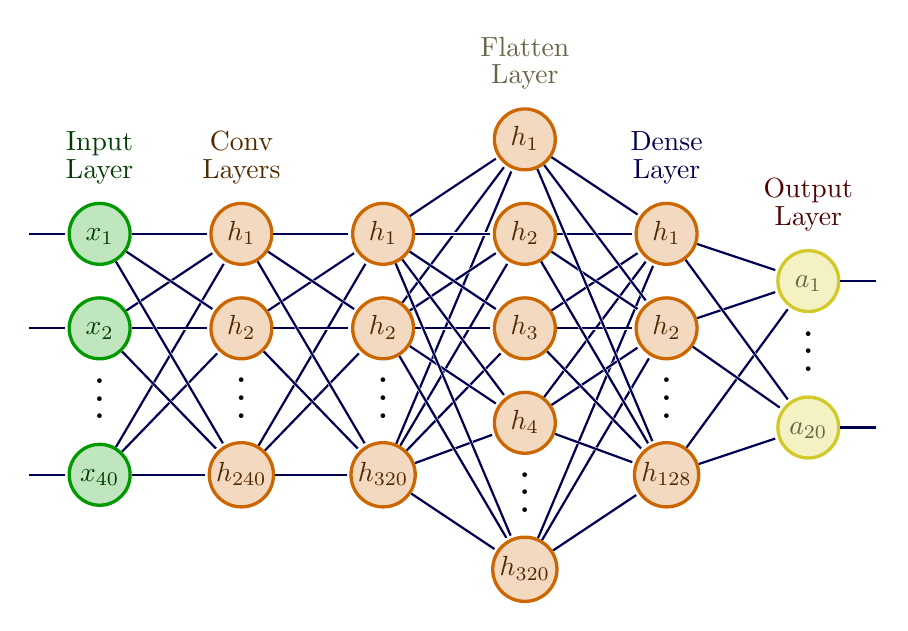
\begin{tikzpicture}[x=1.8cm,y=1.2cm]
    % Input: 4 nodes
    % Conv Layers (2-3): 16, 32 nodes
    % Flatten Layer (4): 320 nodes
    % Dense Layers (5-6): 128, 20 nodes
    \readlist\Nnod{3,3,3,5,3,2} 
    
    \readlist\Nnode{40,240,320,320,128,20}  
    \readlist\Cstr{x,h,h,a,z,y} 
    
    \def\yshift{0.55}
    
    \foreachitem \N \in \Nnod{
        \def\lay{\Ncnt}
        \pgfmathsetmacro\prev{int(\Ncnt-1)}
        \foreach \i [evaluate={
            \c = int(\i==\N);
            \y = \N/2 - \i - \c * \yshift;
            \x = \lay;
            \n = \nstyle;
            \index = (\i<\N ? int(\i) : "\Nnode[\lay]");
        }] in {1,...,\N}{
            \pgfmathsetmacro\nstyle{int(\n==1 ? "input" : (\n==2 ? "conv" : (\n==3 ? "conv" : (\n==4 ? "flat" : (\n==5 ? "dense" : "output")))))}
            \node[\nstyle] (N\lay-\i) at (\x,\y) {$\strut\Cstr[\n]_{\index}$};
            \ifnumcomp{\lay}{>}{1}{
                \foreach \j in {1,...,\Nnod[\prev]}{
                    \draw[white,line width=1.2,shorten >=1] (N\prev-\j) -- (N\lay-\i);
                    \draw[connect] (N\prev-\j) -- (N\lay-\i);
                }
                \ifnum \lay=\Nnodlen
                    \draw[connect] (N\lay-\i) --++ (0.5,0);
                \fi
            }{
                \draw[connect] (0.5,\y) -- (N\lay-\i);
            }
        }
        \path (N\lay-\N) --++ (0,1+\yshift) node[midway,scale=1.6] {$\vdots$};
    }
    \node[above=3,align=center,mydarkgreen] at (N1-1.90) {Input\\[-0.2em]Layer};
    \node[above=3,align=center,mydarkorange] at (N2-1.90) {Conv\\[-0.2em]Layers};
    \node[above=3,align=center,mydarkyellow] at (N4-1.90) {Flatten\\[-0.2em]Layer};
    \node[above=3,align=center,mydarkblue] at (N5-1.90) {Dense\\[-0.2em]Layer};
    \node[above=3,align=center,mydarkred] at (N6-1.90) {Output\\[-0.2em]Layer};
\end{tikzpicture}

\subsection{Représentation des Entrées}
Dans la phase de draft, seules les lignes de départ sont pertinentes. Le plateau est donc représenté comme une grille \(2 \times 5\), où chaque case est encodée par un vecteur à 4 canaux décrivant la présence des différents pions.

\begin{itemize}
    \item Les 4 canaux représentent chaque type de pion (âne, chien, chat, coq).
\end{itemize}

\subsubsection{Dimensions des Entrées}
\begin{itemize}
    \item Pour un plateau unique : \((4, 2, 5)\) (canaux, lignes, colonnes).
    \item Pour un lot de plateaux : \((\text{taille\_batch}, 4, 2, 5)\).
\end{itemize}

\subsection{Représentation des Sorties}
La sortie du réseau encode tous les placements possibles sous forme de liste aplatie de paires \((\text{pion}, \text{colonne})\).

\subsubsection{Taille de la Sortie}
La sortie compte \(4 \times 5 = 20\) placements possibles :
\begin{itemize}
    \item 4 types de pions.
    \item 5 positions possibles sur la ligne de départ.
\end{itemize}

\subsubsection{Encodage des Placements}
Chaque index \(i\) dans la sortie correspond à :
\[
\text{type\_pion} = \lfloor \frac{i}{5} \rfloor, \quad
\text{colonne} = i \bmod 5
\]

\subsection{Architecture du Réseau de Neurones}
L'architecture prend la représentation du plateau de draft en entrée et produit une distribution sur les 20 placements possibles.

\subsubsection{Entrée}
\(\text{Dimensions d'Entrée}: (\text{taille\_batch}, 4, 2, 5)\)

\subsubsection{Couches Convolutionnelles}
\begin{itemize}
    \item \(\text{Conv2D}(4 \rightarrow 16)\) \(\rightarrow\) ReLU
    \item \(\text{Conv2D}(16 \rightarrow 32)\) \(\rightarrow\) ReLU
\end{itemize}

\subsubsection{Couches Entièrement Connectées}
\begin{itemize}
    \item \(\text{Flatten}\)
    \item \(\text{Linear}(2 \times 5 \times 32 \rightarrow 128) \rightarrow \text{ReLU}\)
    \item \(\text{Linear}(128 \rightarrow 20)\)
\end{itemize}

\subsubsection{Sortie}
\[
(\text{taille\_batch}, 20)
\]

\subsection{Mécanisme d'apprentissage spécifique au draft}
L'apprentissage du modèle de draft présente des particularités importantes:

\subsubsection{Signal de récompense différé}
Contrairement au modèle principal où des récompenses peuvent être attribuées à chaque mouvement, le modèle de draft ne reçoit une récompense significative qu'à la fin de la partie:
\begin{itemize}
    \item Récompense positive (\(+100\)) si le joueur gagne la partie.
    \item Récompense négative (\(-100\)) si le joueur perd la partie.
    \item Récompense faiblement négative (\(-5\)) pour les placements invalides.
\end{itemize}

\subsubsection{Stockage des expériences de draft}
Pour faciliter l'apprentissage malgré ce signal de récompense différé, nous maintenons un buffer spécifique pour les expériences de draft:
\begin{verbatim}
self.draft_buffer[color] = []  # Liste pour chaque couleur
# Pour chaque action de draft:
self.draft_buffer[color].append((state_tensor, move_idx, is_valid, next_state_tensor))
\end{verbatim}

À la fin de la partie, ces expériences sont utilisées pour entraîner le modèle de draft avec la récompense appropriée.

\subsection{Interaction entre les modèles}
Les deux modèles (draft et jeu principal) interagissent de la manière suivante:
\begin{itemize}
    \item Le modèle de draft détermine le placement initial des pièces.
    \item Le modèle principal prend le relais pour la phase de jeu proprement dite.
    \item Le résultat final influence l'apprentissage des deux modèles.
\end{itemize}

Cette séparation permet à chaque modèle de se spécialiser dans son domaine spécifique tout en contribuant à l'objectif global de victoire.

\section{Interactions et Améliorations}

\subsection{Coordination entre les systèmes d'IA}
Le succès global de l'agent dépend de la coordination efficace entre les deux systèmes d'IA:
\begin{itemize}
    \item L'IA de draft doit apprendre à créer des positions favorables que l'IA de jeu pourra exploiter.
    \item L'IA de jeu doit être capable d'utiliser efficacement les pièces placées par l'IA de draft.
\end{itemize}

Cette coordination émerge naturellement à travers le processus d'apprentissage, où les récompenses finales guident les deux systèmes vers des stratégies complémentaires.

\subsection{Améliorations potentielles}
Plusieurs pistes d'amélioration pourraient être explorées:

\subsubsection{Architecture des réseaux}
\begin{itemize}
    \item Utilisation d'attention pour mieux capturer les relations entre pièces.
    \item Réseaux résiduels pour faciliter l'entraînement des modèles profonds.
    \item Paramétrage dynamique des couches en fonction de la taille du plateau.
\end{itemize}

\subsubsection{Mécanismes d'apprentissage}
\begin{itemize}
    \item Implémentation de méthodes d'apprentissage plus avancées (A3C, PPO).
    \item Experience replay prioritaire pour favoriser les expériences les plus instructives.
    \item Ajouter des récompenses plus variées que \texttt{victoire/défaite} pour l'agent principal.
\end{itemize}

\subsubsection{Entraînement et évaluation}
\begin{itemize}
    \item Parallélisation de l'entraînement sur plusieurs instances.
    \item Tournois réguliers entre différentes versions des agents pour mesurer les progrès.
    \item Visualisation des représentations internes pour mieux comprendre les stratégies apprises.
\end{itemize}

\end{document}
